\batchmode


\documentclass[letterpaper,hyperref,titlepage]{manual}
\RequirePackage{ifthen}




\usepackage{amsmath}
\usepackage{amssymb} 	
\usepackage[latin1]{inputenc}
\usepackage{textcomp}
\usepackage{fullpage}
\usepackage{graphicx}
\graphicspath{{./graphics/}}
\usepackage{url}
\usepackage{index}
\usepackage{chicago}
\usepackage{xtab}
\usepackage{multirow}

%
\providecommand{\abs}{{\mathrm{abs}}}


\usepackage{courier}
\usepackage{fullpage}
\usepackage{color}  


\definecolor{darkorange}{rgb}{.71,0.21,0.01}
\definecolor{darkgreen}{rgb}{.12,.54,.11}


\usepackage[    breaklinks=true,    colorlinks=true,  urlcolor=blue,  linkcolor=darkorange,  citecolor=darkgreen,  ]{hyperref}


\sloppy

%
\providecommand{\fixme}[1]{
\textcolor{red}{
{\fbox{ {\bf FIX}
\ensuremath{\blacktriangleright \blacktriangleright \blacktriangleright}}
{\bf #1}
\fbox{\ensuremath{ \blacktriangleleft \blacktriangleleft \blacktriangleleft }
} } }
} 


\definecolor{orange}{cmyk}{0,0.4,0.8,0.2}
\usepackage{listings}
\lstset{
  language=Python,
  basicstyle=\small\ttfamily ,
  commentstyle=\ttfamily\color{blue},
  stringstyle=\ttfamily\color{orange},
  showstringspaces=false,
  breaklines=true,
  postbreak = \ \dots
}

%
\providecommand{\pypedal}{PyPedal}%
\providecommand{\PyPedal}{PyPedal}   % Only beginning of sentence, otherwise use \pypedal{}%
\providecommand{\PYPEDAL}{PyPedal}%
\providecommand{\python}{Python} 

%
\providecommand{\remark}[1]{} 


\title{A Manual for use of PyPedal\\A software package for pedigree analysis}
\author{John B. Cole}
\authoraddress{Animal Improvement Programs Laboratory, Agricultural Research Service, United States Department of Agriculture, Room 306 Bldg 005 BARC-West, 10300 Baltimore Avenue, Beltsville, MD 20705-2350}


\date{November 29, 2005 \\Revised \today}                   % update before release!
                                

\release{2.0.0b23}              % (software) release version;
\setshortversion{2.0}           % this is used to define the \version macro
\makeindex                      % tell \index to actually write the .idx file
\newindex{func}{fdx}{fnd}{Function Index}





\pagecolor[gray]{.7}

\usepackage[latin1]{inputenc}



\makeatletter
\AtBeginDocument{\makeatletter
\input /home/jcole/pypedal/PyPedal/doc/pypedal.aux
\makeatother
}

\makeatletter
\count@=\the\catcode`\_ \catcode`\_=8 
\newenvironment{tex2html_wrap}{}{}%
\catcode`\<=12\catcode`\_=\count@
\newcommand{\providedcommand}[1]{\expandafter\providecommand\csname #1\endcsname}%
\newcommand{\renewedcommand}[1]{\expandafter\providecommand\csname #1\endcsname{}%
  \expandafter\renewcommand\csname #1\endcsname}%
\newcommand{\newedenvironment}[1]{\newenvironment{#1}{}{}\renewenvironment{#1}}%
\let\newedcommand\renewedcommand
\let\renewedenvironment\newedenvironment
\makeatother
\let\mathon=$
\let\mathoff=$
\ifx\AtBeginDocument\undefined \newcommand{\AtBeginDocument}[1]{}\fi
\newbox\sizebox
\setlength{\hoffset}{0pt}\setlength{\voffset}{0pt}
\addtolength{\textheight}{\footskip}\setlength{\footskip}{0pt}
\addtolength{\textheight}{\topmargin}\setlength{\topmargin}{0pt}
\addtolength{\textheight}{\headheight}\setlength{\headheight}{0pt}
\addtolength{\textheight}{\headsep}\setlength{\headsep}{0pt}
\setlength{\textwidth}{349pt}
\newwrite\lthtmlwrite
\makeatletter
\let\realnormalsize=\normalsize
\global\topskip=2sp
\def\preveqno{}\let\real@float=\@float \let\realend@float=\end@float
\def\@float{\let\@savefreelist\@freelist\real@float}
\def\liih@math{\ifmmode$\else\bad@math\fi}
\def\end@float{\realend@float\global\let\@freelist\@savefreelist}
\let\real@dbflt=\@dbflt \let\end@dblfloat=\end@float
\let\@largefloatcheck=\relax
\let\if@boxedmulticols=\iftrue
\def\@dbflt{\let\@savefreelist\@freelist\real@dbflt}
\def\adjustnormalsize{\def\normalsize{\mathsurround=0pt \realnormalsize
 \parindent=0pt\abovedisplayskip=0pt\belowdisplayskip=0pt}%
 \def\phantompar{\csname par\endcsname}\normalsize}%
\def\lthtmltypeout#1{{\let\protect\string \immediate\write\lthtmlwrite{#1}}}%
\newcommand\lthtmlhboxmathA{\adjustnormalsize\setbox\sizebox=\hbox\bgroup\kern.05em }%
\newcommand\lthtmlhboxmathB{\adjustnormalsize\setbox\sizebox=\hbox to\hsize\bgroup\hfill }%
\newcommand\lthtmlvboxmathA{\adjustnormalsize\setbox\sizebox=\vbox\bgroup %
 \let\ifinner=\iffalse \let\)\liih@math }%
\newcommand\lthtmlboxmathZ{\@next\next\@currlist{}{\def\next{\voidb@x}}%
 \expandafter\box\next\egroup}%
\newcommand\lthtmlmathtype[1]{\gdef\lthtmlmathenv{#1}}%
\newcommand\lthtmllogmath{\dimen0\ht\sizebox \advance\dimen0\dp\sizebox
  \ifdim\dimen0>.95\vsize
   \lthtmltypeout{%
*** image for \lthtmlmathenv\space is too tall at \the\dimen0, reducing to .95 vsize ***}%
   \ht\sizebox.95\vsize \dp\sizebox\z@ \fi
  \lthtmltypeout{l2hSize %
:\lthtmlmathenv:\the\ht\sizebox::\the\dp\sizebox::\the\wd\sizebox.\preveqno}}%
\newcommand\lthtmlfigureA[1]{\let\@savefreelist\@freelist
       \lthtmlmathtype{#1}\lthtmlvboxmathA}%
\newcommand\lthtmlpictureA{\bgroup\catcode`\_=8 \lthtmlpictureB}%
\newcommand\lthtmlpictureB[1]{\lthtmlmathtype{#1}\egroup
       \let\@savefreelist\@freelist \lthtmlhboxmathB}%
\newcommand\lthtmlpictureZ[1]{\hfill\lthtmlfigureZ}%
\newcommand\lthtmlfigureZ{\lthtmlboxmathZ\lthtmllogmath\copy\sizebox
       \global\let\@freelist\@savefreelist}%
\newcommand\lthtmldisplayA{\bgroup\catcode`\_=8 \lthtmldisplayAi}%
\newcommand\lthtmldisplayAi[1]{\lthtmlmathtype{#1}\egroup\lthtmlvboxmathA}%
\newcommand\lthtmldisplayB[1]{\edef\preveqno{(\theequation)}%
  \lthtmldisplayA{#1}\let\@eqnnum\relax}%
\newcommand\lthtmldisplayZ{\lthtmlboxmathZ\lthtmllogmath\lthtmlsetmath}%
\newcommand\lthtmlinlinemathA{\bgroup\catcode`\_=8 \lthtmlinlinemathB}
\newcommand\lthtmlinlinemathB[1]{\lthtmlmathtype{#1}\egroup\lthtmlhboxmathA
  \vrule height1.5ex width0pt }%
\newcommand\lthtmlinlineA{\bgroup\catcode`\_=8 \lthtmlinlineB}%
\newcommand\lthtmlinlineB[1]{\lthtmlmathtype{#1}\egroup\lthtmlhboxmathA}%
\newcommand\lthtmlinlineZ{\egroup\expandafter\ifdim\dp\sizebox>0pt %
  \expandafter\centerinlinemath\fi\lthtmllogmath\lthtmlsetinline}
\newcommand\lthtmlinlinemathZ{\egroup\expandafter\ifdim\dp\sizebox>0pt %
  \expandafter\centerinlinemath\fi\lthtmllogmath\lthtmlsetmath}
\newcommand\lthtmlindisplaymathZ{\egroup %
  \centerinlinemath\lthtmllogmath\lthtmlsetmath}
\def\lthtmlsetinline{\hbox{\vrule width.1em \vtop{\vbox{%
  \kern.1em\copy\sizebox}\ifdim\dp\sizebox>0pt\kern.1em\else\kern.3pt\fi
  \ifdim\hsize>\wd\sizebox \hrule depth1pt\fi}}}
\def\lthtmlsetmath{\hbox{\vrule width.1em\kern-.05em\vtop{\vbox{%
  \kern.1em\kern0.8 pt\hbox{\hglue.17em\copy\sizebox\hglue0.8 pt}}\kern.3pt%
  \ifdim\dp\sizebox>0pt\kern.1em\fi \kern0.8 pt%
  \ifdim\hsize>\wd\sizebox \hrule depth1pt\fi}}}
\def\centerinlinemath{%
  \dimen1=\ifdim\ht\sizebox<\dp\sizebox \dp\sizebox\else\ht\sizebox\fi
  \advance\dimen1by.5pt \vrule width0pt height\dimen1 depth\dimen1 
 \dp\sizebox=\dimen1\ht\sizebox=\dimen1\relax}

\def\lthtmlcheckvsize{\ifdim\ht\sizebox<\vsize 
  \ifdim\wd\sizebox<\hsize\expandafter\hfill\fi \expandafter\vfill
  \else\expandafter\vss\fi}%
\providecommand{\selectlanguage}[1]{}%
\makeatletter \tracingstats = 1 
\providecommand{\Beta}{\textrm{B}}
\providecommand{\Mu}{\textrm{M}}
\providecommand{\Kappa}{\textrm{K}}
\providecommand{\Rho}{\textrm{R}}
\providecommand{\Epsilon}{\textrm{E}}
\providecommand{\Chi}{\textrm{X}}
\providecommand{\Iota}{\textrm{J}}
\providecommand{\omicron}{\textrm{o}}
\providecommand{\Zeta}{\textrm{Z}}
\providecommand{\Eta}{\textrm{H}}
\providecommand{\Nu}{\textrm{N}}
\providecommand{\Omicron}{\textrm{O}}
\providecommand{\Tau}{\textrm{T}}
\providecommand{\Alpha}{\textrm{A}}


\begin{document}
\pagestyle{empty}\thispagestyle{empty}\lthtmltypeout{}%
\lthtmltypeout{latex2htmlLength hsize=\the\hsize}\lthtmltypeout{}%
\lthtmltypeout{latex2htmlLength vsize=\the\vsize}\lthtmltypeout{}%
\lthtmltypeout{latex2htmlLength hoffset=\the\hoffset}\lthtmltypeout{}%
\lthtmltypeout{latex2htmlLength voffset=\the\voffset}\lthtmltypeout{}%
\lthtmltypeout{latex2htmlLength topmargin=\the\topmargin}\lthtmltypeout{}%
\lthtmltypeout{latex2htmlLength topskip=\the\topskip}\lthtmltypeout{}%
\lthtmltypeout{latex2htmlLength headheight=\the\headheight}\lthtmltypeout{}%
\lthtmltypeout{latex2htmlLength headsep=\the\headsep}\lthtmltypeout{}%
\lthtmltypeout{latex2htmlLength parskip=\the\parskip}\lthtmltypeout{}%
\lthtmltypeout{latex2htmlLength oddsidemargin=\the\oddsidemargin}\lthtmltypeout{}%
\makeatletter
\if@twoside\lthtmltypeout{latex2htmlLength evensidemargin=\the\evensidemargin}%
\else\lthtmltypeout{latex2htmlLength evensidemargin=\the\oddsidemargin}\fi%
\lthtmltypeout{}%
\makeatother
\setcounter{page}{1}
\onecolumn

% !!! IMAGES START HERE !!!

\stepcounter{chapter}
\stepcounter{section}
{\newpage\clearpage
\lthtmlinlinemathA{tex2html_wrap_inline8481}%
$ A$%
\lthtmlinlinemathZ
\lthtmlcheckvsize\clearpage}

{\newpage\clearpage
\lthtmlinlinemathA{tex2html_wrap_inline8485}%
$ T$%
\lthtmlinlinemathZ
\lthtmlcheckvsize\clearpage}

{\newpage\clearpage
\lthtmlinlinemathA{tex2html_wrap_inline8487}%
$ D$%
\lthtmlinlinemathZ
\lthtmlcheckvsize\clearpage}

{\newpage\clearpage
\lthtmlinlinemathA{tex2html_wrap_inline8489}%
$ A=TDT'$%
\lthtmlinlinemathZ
\lthtmlcheckvsize\clearpage}

\stepcounter{section}
\stepcounter{section}
\stepcounter{section}
\stepcounter{chapter}
\stepcounter{section}
{\newpage\clearpage
\lthtmlfigureA{xtabular359}%
\begin{xtabular}{llp{4in}}
	elementtree & Lightweight XML processing & \url{http://effbot.org/zone/element-index.htm}\\
	Graphviz & Draw directed graphs & \url{http://www.research.att.com/sw/tools/graphviz/}\\
	matplotlib & Plotting, matrix visualization & \url{http://matplotlib.sourceforge.net/}\\
	NetworkX & Network analysis & \url{https://networkx.lanl.gov/}\\
	NumPy & Array manipulation & \url{http://www.numpy.org/}\\
	PIL & Image processing & \url{http://effbot.org/zone/pil-index.htm}\\
	pydot & Interface to Graphviz & \url{http://dkbza.org/pydot.html}\\
	PyGraphviz & Interface to Graphviz & \url{https://networkx.lanl.gov/wiki/pygraphviz}\\
	pyparsing & Text parsing & \url{http://pyparsing.sourceforge.net/}\\
	pysqlite & Interface to SQLite & \url{http://initd.org/tracker/pysqlite}\\
	PythonDoc & Generate API documentation & \url{http://effbot.org/zone/pythondoc.htm}\\
	ReportLab & Generate PDF documents & \url{http://www.reportlab.org/}\\
	SQLite & Lightweight SQL database & \url{http://www.sqlite.org/}\\
	testoob & Advanced unit testing & \url{http://testoob.sourceforge.net/}\\
    \end{xtabular}%
\lthtmlfigureZ
\lthtmlcheckvsize\clearpage}

\stepcounter{section}
\stepcounter{section}
\stepcounter{subsection}
\stepcounter{subsection}
{\newpage\clearpage
\lthtmlinlinemathA{tex2html_wrap_inline8513}%
$ \blacktriangleright \blacktriangleright \blacktriangleright$%
\lthtmlinlinemathZ
\lthtmlcheckvsize\clearpage}

{\newpage\clearpage
\lthtmlinlinemathA{tex2html_wrap_inline8516}%
$ \blacktriangleleft \blacktriangleleft \blacktriangleleft $%
\lthtmlinlinemathZ
\lthtmlcheckvsize\clearpage}

\stepcounter{subsubsection}
\stepcounter{subsubsection}
\stepcounter{section}
\stepcounter{chapter}
\stepcounter{section}
\stepcounter{section}
\stepcounter{section}
\stepcounter{section}
{\newpage\clearpage
\lthtmlfigureA{xtabular663}%
\begin{xtabular}
% latex2html id marker 663
{l|l|p{4in}}
	alleles\_sepchar  & '/'          & The character separating the two alleles in an animal's allelotype. \var{alleles\_sepchar} CANNOT be the same as \var{sepchar}! \\
	animal\_type  & 'new'           & Indicates which animal class should be used to instantiate animal records, \class{NewAnimal} or \class{LightAnimal} (`new'|`light'). \\
	counter          & 1000         & How often should  PyPedal{} write a note to the screen when reading large pedigree files. \\
	database\_name   & 'pypedal'    & The name of the database to be used when using the \module{pyp\_reports} nodule. \\
	dbtable\_name     & filetag      & The name of the database table to which the current pedigree will be written when using the \module{pyp\_reports} module. \\
	default\_fontsize & 10           & Specifies the default font size used in \module{pyp   \_graphics}. If the font size cannot be cast to an integer, it is set to the default value of 10. Font sizes less than 1 are set to the default of 10. \\
	default\_report   & filetag      & Default report name for use by \module{pyp\_reports}. \\
	default\_unit     & 'inch'       & The default unit of measurement for report generation ('cm'|'inch'). \\
	debug\_messages  & 0            & Indicates whether or not PyPedal{} should print debugging information. \\
	f\_computed       & 0            & Indicates whether or not coefficients of inbreeding  have been computed for animals in the current pedigree.  If the pedigree format string includes \character{f} this will be set to 1; it is also set to 1 on a successful return from \function{pyp\_nrm/inbreeding()}. \\
	file\_io         & 1            & When true, routines that can write results to output files will do so and put messages in the program log to that effect. \\
	filetag          & pedfile      & \var{filetag} is a descriptive label attached to output files created when processing a pedigree.  By default the filetag is based on \var{pedfile}, minus its file extension. \\
	form\_nrm        & 0            & Indicates whether or not to form a NRM and bind it to the pedigree as an instance of a \class{NewAMatrix} object. \\
	gen\_coeff       & 0            & When nonzero, calculate generation coefficients using the method of Pattie \citeyear{Pattie1965} and store them in the \member{gen\_coeff} attribute of a \class{NewAnimal} object.  The inferred generation stored in the \member{igen} attribute will be the \member{gen\_coeff} rounded to the nearest 0.5.  When zero, the \member{gen\_coeff} is -999. \\
	log\_long\_filenames & 0        & When nonzero, long logfile names will be used, which means that log file names will include datestamps. \\
	log\_ped\_lines  & 0            & When $>$\  0 indicates how many lines read from the pedigree file should be printed in the log file for debugging purposes. \\
	logfile          & filetag.log  & The name of the file to which PyPedal{} should write messages about its progress. \\
	messages         & 'verbose'    & How chatty PyPedal{} should be with respect to messages to the user.  'verbose' indicates that all status messages will be written to STDOUT, while 'quiet' suppresses all output to STDOUT. \\
	missing\_bdate    & '01011900'   & Default birth date. \\
	missing\_breed    & 'Unknown'    & Default breed name.\\
	missing\_byear    & 1900         & Default birth year.\\
	missing\_name     & 'Unknown'    & Default animal name.\\
	missing\_parent  & 0            & Indicates what code is used to identify missing/unknown parents in the pedigree file. \\
	newanimal\_caller  & 'loader'   & Internal parameter needed for addanimal() to work correctly with ASD pedigrees. \\
	nrm\_format      & 'text'       & Format to use when writing an NRM to a file ('text'|'binary'). Array elements in text files are separated by \var{sepchar}.\\
	nrm\_method      & 'nrm'        & Specifies that an NRM formed from the current pedigree as an instance of a \class{NewAMatrix} object should ('frm') or should not ('nrm') be corrected for parental inbreeding. \\
	paper_size       & 'letter'     & Default paper size for printed reports ('A4'|'letter'). \\
	pedcomp          & 0            & When 1, calculate pedigree completeness using pedcomp\_gens generations of pedigree. \\
	pedcomp\_gens    & 3            & Number of generations of pedigree to use when calculating pedigree completeness. \\
	pedfile          & None         & File from which pedigree is read; must provided unless you are simulating a pedigree. Defaults to 'simulated_pedigree' for simulated pedigrees. \\
	pedformat        & 'asd'        & See \ref{sec:pedigree-format-codes} for details. \\
	pedname          & 'Untitled'   & A name/title for your pedigree. \\
	pedgree\_is\_renumbered & 0     & Indicates whether or not the pedigree has been renumbered. \\
	pedigree\_summary & 1           & Indicates whether or not the pedigree loading details and summary are printed to STDOUT.  Output is only written if \var{message} is set to `verbose'. \\
	renumber         & 0            & Renumber the pedigree after reading from file (0/1). \\
	sepchar          & ' '          & The character separating columns of input in the pedfile. \\
	set\_ancestors   & 0            & Iterate over the pedigree to assign ancestors lists to parents in the pedigree (0/1). \\
	set\_alleles     & 0            & Assign alleles for use in gene-drop simulations (0/1). \\
	set\_generations & 0            & Iterate over the pedigree to infer generations (0/1). \\
	set\_offspring   & 0            & Assigns offspring to their parent(s)'s unknown sex offspring list. \\
	set\_sexes       & 0            & Iterate over the pedigree to assign sexes to all animals in the pedigree (0/1). \\
	simulate\_fs     & 0            & Flag indicating whether or not full-sib matings are allowed. \\
	simulate\_g      & 3            & Number of distinct generations in the simulated pedigree. \\
	simulate\_ir     & 0.0          & Immigration rate, the rate at which new founders with unknown parents enter the population. \\
	simulate\_mp     & 0            & Flag indicating whether or not simulated animals may have missing parents. \\
	simulate\_n      & 15           & Total number of animals in simulated pedigree, including founders. \\
	simulate\_nd     & 4            & Number of initial founder dams in pedigree. \\
	simulate\_ns     & 4            & Number of initial founder sires in pedigree. \\
	simulate\_pedigree & 0          & Option to simulate a pedigree rather that load one from a file. All other simulation-related variables are ignored when this is not set to 1. \\
	simulate\_pmd    & 100          & Maximum number of draws allowed when trying to sample parents that comply with all restrictions. \\
	simulate\_po     & 0            & Flag indicating whether or not parent-offspring matings are allowed. \\
	simulate\_save   & 0            & Flag indicating whether or not the simulated pedigree should be written to a file after it is created. \\
	simulate\_sr     & 0.5          & Sex ratio in simulated pedigree; < 0.5 gives more females, > 0.5 gives more males. \\
	slow\_reorder    & 1            & Option to override the slow, but more correct, reordering routine used by PyPedal by default (0/1).  ONLY CHANGE THIS IF YOU REALLY UNDERSTAND WHAT IT DOES!  Careless use of this option can lead to erroneous results. \\
    \end{xtabular}%
\lthtmlfigureZ
\lthtmlcheckvsize\clearpage}

\stepcounter{subsection}
\stepcounter{section}
\stepcounter{subsection}
{\newpage\clearpage
\lthtmlfigureA{xtabular753}%
\begin{xtabular}{l|p{4in}}
	a & animal ('a' or 'A' REQUIRED)\\
	s & sire ('s' or 'S' REQUIRED)\\
	d & dam ('d' or 'D' REQUIRED)\\
	y & birthyear (YYYY)\\
	e & age\\
	f & coefficient of inbreeding\\
	g & generation\\
	h & herd\\
	l & alive (1) or dead (0)\\
	n & name\\
	p & Pattie's \citeyear{Pattie1965} generation coefficient\\
	r & breed\\
	u & user-defined field (string)\\
	b & birthdate in "MMDDYYYY" format\\
	x & sex\\
	A & animal ID as a string (cannot contain \samp{sepchar})\\
	S & sire ID as a string (cannot contain \samp{sepchar})\\
	D & dam ID as a string (cannot contain \samp{sepchar})\\
	H & herd as a string (cannot contain \samp{sepchar})\\
	L & alleles (two alleles separated by a non-null character)\\
	Z & indicates a column that should be skipped (one allowed per pedigree)\\
    \end{xtabular}%
\lthtmlfigureZ
\lthtmlcheckvsize\clearpage}

\stepcounter{section}
\stepcounter{subsection}
\stepcounter{section}
\stepcounter{section}
{\newpage\clearpage
\lthtmlinlinemathA{tex2html_wrap_inline8564}%
$ >$%
\lthtmlinlinemathZ
\lthtmlcheckvsize\clearpage}

{\newpage\clearpage
\lthtmlinlinemathA{tex2html_wrap_inline8566}%
$ <$%
\lthtmlinlinemathZ
\lthtmlcheckvsize\clearpage}

{\newpage\clearpage
\lthtmlpictureA{tex2html_wrap8572}%
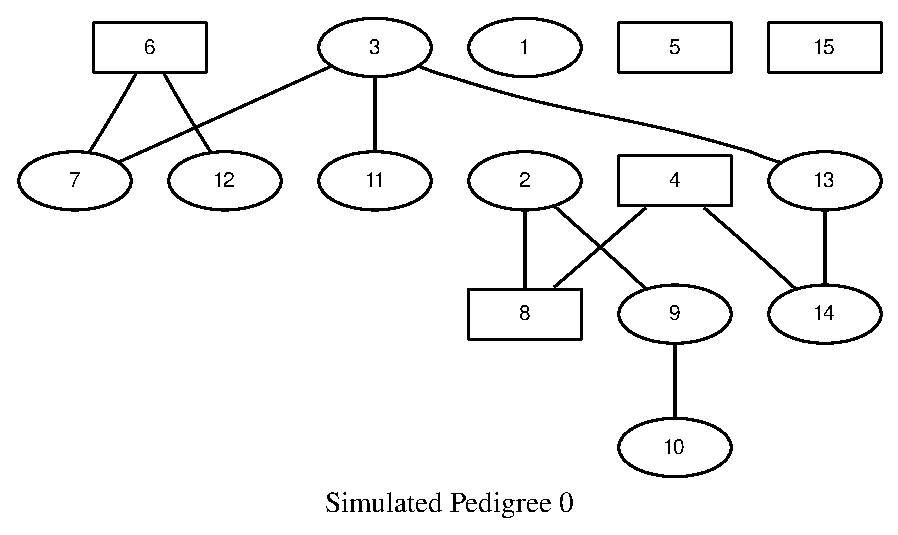
\includegraphics[width=4in]{simulatedPedigree.eps}%
\lthtmlpictureZ
\lthtmlcheckvsize\clearpage}

\stepcounter{chapter}
\stepcounter{section}
{\newpage\clearpage
\lthtmlfigureA{xtabular910}%
\begin{xtabular}{l|p{1in}|p{3in}}
    Input & db & Load an ASDx-formatted data from an SQLite database \\
     & fromgraph & Load a pedigree from an instance of an XDiGraph object (not a file) \\
     & gedcomfile & Load a pedigree from a GEDCOM 5.5 file \\
     & graphfile & Load a pedigree from an adjacency list using the read_adjlist() function from the NetworkX module \\
     & simulate & Simulate a pedigree rathen that loading it from a file \\
     & textstream & Load a pedigree from a string contaiing animal records \\
    Output & save & Save a pedigree to a user-specified file \\
     & savedb & Save a pedigree to a database table \\
     & savegedcom & Save a pedigree to a GEDCOM 5.5 file \\
     & savegraph & Save a pedigree to a file as an adjacency list \\
    \end{xtabular}%
\lthtmlfigureZ
\lthtmlcheckvsize\clearpage}

\stepcounter{section}
\stepcounter{subsection}
\stepcounter{subsection}
\stepcounter{subsection}
\stepcounter{subsection}
\stepcounter{subsection}
\stepcounter{section}
\stepcounter{subsection}
\stepcounter{subsection}
\stepcounter{subsection}
\stepcounter{subsection}
\stepcounter{chapter}
\stepcounter{section}
\stepcounter{subsection}
{\newpage\clearpage
\lthtmlfigureA{xtabular1140}%
\begin{xtabular}
% latex2html id marker 1140
{l|l|l|p{2.5in}}
        age & -999 & -999 & The animal's age based on the global \texttt{BASE_DEMOGRAPHIC_YEAR} defined in \module{pyp_demog}. If the \emph{by} is unknown, the inferred generation is used.  If the inferred generation is unknown, the age is set to -999. \\
        alive & \texttt{'0'} & \texttt{'0'} & Flag indicating whether or not the animal is alive: \texttt{'0'} = dead, \texttt{'1'} = alive. \\
        alleles & $['', '']$\  & $['', '']$\  & Alleles used for gene dropping. \\
        ancestor & \texttt{'0'} & \texttt{'0'} & Flag indicating whether or not the animal has offspring: \texttt{'0'} = has no offspring, \texttt{'1'} = has offspring. The flags are set by calling \function{pyp\_utils.set\_ancestor\_flag()} and passing it a renumbred pedigree. \\
        animalID & animal ID & animal ID $\mapsto$\  \emph{integer} & Animal's ID. Animal IDs change when a pedigree is renumbered. IDs must be provided for all animals in a pedigree file. When strings are provided for animal  IDs using the \texttt{ASD} pedigree format code they are converted to integral animal IDs using the \method{string_to_int()} method.\\
        bd & \texttt{missing_bdate} & \texttt{missing_bdate} & The animal's birthdate in \emph{MMDDYY} format. \\
        breed & \texttt{missing_breed} & \texttt{missing_breed} & The animal's breed as a string. \\
        by & \texttt{missing_byear} & \texttt{missing_byear} & The animal's birthyear in \emph{YYYY} format. Default values set in \texttt{this typeface} are  PyPedal{} options which are described in detail in Section \ref{sec:pypedal-options}.\\
        damID & dam ID & dam ID $\mapsto$\  \emph{integer} & Dam's ID. When strings are provided for animal  IDs using the \texttt{ASD} pedigree format code they are converted to integral animal IDs using the \method{string_to_int()} method. \\
        damName & dam ID & dam ID & The name of the animal's dam. \\
        daus & $\{\}$\  & $\{\}$\  & Dictionary containing all known daughters of an animal. The keys and values are the animal IDs for each offspring. When the pedigree is renumbered, keys are updated to correspond to the renumbered IDs for each offspring. \\
        fa & 0.0 & 0.0 & The animal's coefficient of inbreeding. \\
        founder & \texttt{'n'} & \texttt{'n'} & Character indicating whether or not the animal is a founder (had unknown parents): \texttt{'n'} = not a founder (one or both parents known), \texttt{'y'} = founder (parents unknown).\\
        gen & -999 & -999 & Generation to which the animal belongs. \\
        gencoeff & -999.0 & -999.0 & Pattie's \citeyear{Pattie1965} generation coefficient. \\
        herd & \texttt{missing_herd} $\mapsto$\  \emph{integer} & \texttt{missing_herd} $\mapsto$\  \emph{integer} & The ID of the herd to which the animal belongs. \\
        igen & -999 & -999 & Generation inferred by \function{pyp\_utils.set\_generation()}. \\
        name & animal ID & animal ID & The animal's name. This attribute is quite useful in \texttt{ASD} pedigrees. and less so in \texttt{asd} pedigrees. \\
        originalHerd & herd & herd & The original herd ID to which an animal belonged before the herd was converted from a string to an integer; most useful with the \texttt{'H'} pedigree format code. \\
        originalID & animalID & animal ID $\mapsto$\  \emph{integer} & Original ID assigned to an animal. It will not change when the pedigree is renumbered. \\
        paddedID & \texttt{animalID} $\mapsto$\  \emph{integer} & \texttt{animalID} $\mapsto$\  \emph{integer} & The animal ID padded to fifteen digits, with the birthyear (or 1950 if the birth year is unknown) prepended.  The order of elements is: birthyear, animalID,count of zeros, zeros. Used to create alleles for gene dropping. \\
        pedcomp & -999.9 & -999.9 & Pedigree completeness as described in Section \ref{sec:methodology-pedigre-completeness}. \\
        renumberedID & -999 & -999 & ID assigned to an animal when the pedigree is renumbered. The default value indicates that the pedigree has not been renumbered using PyPedal{}.\\
        sex & \texttt{'u'} & \texttt{'u'} & The sex of the animal: \texttt{'m'} = male, \texttt{'f'} = female, \texttt{'u'} = unknown/not provided. \\
        sireID & sire ID & sire ID $\mapsto$\  \emph{integer} & Sire's ID. When strings are provided for animal  IDs using the \texttt{ASD} pedigree format code they are converted to integral animal IDs using the \method{string_to_int()} method. \\
        sireName & sireID & sireID & The name of the animal's sire. \\
        sons & $\{\}$\  & $\{\}$\  & Dictionary containing all known sons of an animal. The keys and values are the animal IDs for each offspring. When the pedigree is renumbered, keys are updated to correspond to the renumbered IDs for each offspring.\\
        unks & $\{\}$\  & $\{\}$\  & Dictionary containing all offspring of an animal with unknown sex. The keys and values are the animal IDs for each offspring. When the pedigree is renumbered, keys are updated to correspond to the renumbered IDs for each offspring. \\
    \end{xtabular}%
\lthtmlfigureZ
\lthtmlcheckvsize\clearpage}

{\newpage\clearpage
\lthtmlfigureA{xtabular1214}%
\begin{xtabular}{l|p{4in}}
        \_\_init\_\_ & Initializes a \class{NewAnimal} object and returns an instance of a \class{NewAnimal} object. \\
        printme & Prints a summary of the data stored in a \class{NewAnimal} object. \\
        stringme & Returns the data stored in a \class{NewtAnimal} object as a string. \\
        dictme & Returns the data stored in a \class{NewtAnimal} object as a dictionary whose keys are attribute names and whose values are attribute values. \\
        trap & Checks for common errors in \class{NewtAnimal} objects. \\
        pad\_id & Takes an animal ID, pads it to fifteen digits, and prepends the birthyear. The order of elements is: birthyear, animalID, count of zeros, zeros. The padded ID is used for reordering the pedigree with the \function{fast\_reorder} routine. \\
        string\_to\_int & Takes an animal ID as a string and returns a hash. The algorithm used is taken from "Character String Keys" in "Data Structures and Algorithms with Object-Oriented Design Patterns in Python" by Bruno R. Preiss: \url{http://www.brpreiss.com/books/opus7/html/page220.html#progstrnga}. \\
    \end{xtabular}%
\lthtmlfigureZ
\lthtmlcheckvsize\clearpage}

\stepcounter{subsection}
{\newpage\clearpage
\lthtmlfigureA{xtabular1242}%
\begin{xtabular}{l|l|p{4in}}
        animalID & animal ID & Animal's ID. \\
        by & \texttt{missing_byear} & The animal's birthyear in \emph{YYYY} format. \\
        damID & 0 & Dam's ID. \\
        originalID & animalID & Original ID assigned to an animal. It will not change when the pedigree is renumbered. \\
        renumberedID & animalID & Renumbered ID assigned to an animal. It is assigned by the renumbering routine. \\
        sex & \texttt{'u'} & The sex of the animal: \texttt{'m'} = male, \texttt{'f'} = female, \texttt{'u'} = unknown. \\
        sireID & 0 & Sire's ID. \\
    \end{xtabular}%
\lthtmlfigureZ
\lthtmlcheckvsize\clearpage}

{\newpage\clearpage
\lthtmlfigureA{xtabular1265}%
\begin{xtabular}{l|p{4in}}
        \_\_init\_\_ & Initializes a \class{LightAnimal} object and returns an instance of a \class{LightAnimal} object. \\
        printme & Prints a summary of the data stored in a \class{LightAnimal} object. \\
        stringme & Returns the data stored in a \class{LightAnimal} object as a string. \\
        dictme & Returns the data stored in a \class{LightAnimal} object as a dictionary whose keys are attribute names and whose values are attribute values. \\
        trap & Checks for common errors in \class{LightAnimal} objects. \\
        pad\_id & Takes an animal ID, pads it to fifteen digits, and prepends the birthyear. The order of elements is: birthyear, animalID, count of zeros, zeros. The padded ID is used for reordering the pedigree with the \function{fast\_reorder} routine. \\
        string\_to\_int & Takes an animal ID as a string and returns a hash. The algorithm used is taken from "Character String Keys" in "Data Structures and Algorithms with Object-Oriented Design Patterns in Python" by Bruno R. Preiss: \url{http://www.brpreiss.com/books/opus7/html/page220.html#progstrnga}. \\
    \end{xtabular}%
\lthtmlfigureZ
\lthtmlcheckvsize\clearpage}

\stepcounter{subsection}
{\newpage\clearpage
\lthtmlfigureA{xtabular1294}%
\begin{xtabular}{l|l|p{4in}}
        animalID & animal ID & Animal's ID. \\
        damID & 0 & Dam's ID. \\
        gen & 0 & Generation to which the animal belongs. \\
        sex & \texttt{'u'} & The sex of the animal: \texttt{'m'} = male, \texttt{'f'} = female, \texttt{'u'} = unknown. \\
        sireID & 0 & Sire's ID. \\
    \end{xtabular}%
\lthtmlfigureZ
\lthtmlcheckvsize\clearpage}

{\newpage\clearpage
\lthtmlfigureA{xtabular1313}%
\begin{xtabular}{l|p{4in}}
        \_\_init\_\_ & Initializes a \class{SimAnimal} object and returns an instance of a \class{SimAnimal} object. \\
        printme & Prints a summary of the data stored in a \class{SimAnimal} object. \\
        stringme & Returns the data stored in a \class{SimAnimal} object as a string. \\
    \end{xtabular}%
\lthtmlfigureZ
\lthtmlcheckvsize\clearpage}

\stepcounter{section}
{\newpage\clearpage
\lthtmlfigureA{xtabular1335}%
\begin{xtabular}
% latex2html id marker 1335
{l|l|p{4in}}
        kw & \texttt{kw} & Keyword dictionary. \\
	pedigree & $[]$\  & A list of \class{NewAnimal} objects. \\
        metadata & $\{\}$\  & A \class{PedigreeMetadata} object. \\
        idmap & $\{\}$\  & Dictionary for mapping original IDs to renumbered IDs (\ref{sec:methodology-id-mapping}). \\
        backmap & $\{\}$\  & Dictionary for mapping renumbered IDs to original IDs (\ref{sec:methodology-id-mapping}). \\
        namemap & $\{\}$\  & Dictionary for mapping names to original IDs (\ref{sec:methodology-id-mapping}). \\
        namebackmap & $\{\}$\  & Dictionary for mapping original IDs to names (\ref{sec:methodology-id-mapping}). \\
        starline & \texttt{'*'*80} & Convenience string. \\
        nrm & None & An instance of a \class{NewAMatrix} object. \\
    \end{xtabular}%
\lthtmlfigureZ
\lthtmlcheckvsize\clearpage}

{\newpage\clearpage
\lthtmlfigureA{xtabular1359}%
\begin{xtabular}{l|p{4in}}
        \_\_init\_\_ & Initializes and returns a \class{NewPedigree} object. \\
        addanimal & Adds a new animal of class \class{NewAnimal} to the pedigree. \textbf{Note:} This function should be used by \class{NewPedigree} methods only, not userspace routines. Improper use of \method{addanimal} may result in data loss or corruption. You have been warned. \\
        delanimal & Deletes an animal from the pedigree. Note that this method DOES not update the metadata attached to the pedigree and should only be used if that is not important. \textbf{Note:} This function should be used by \class{NewPedigree} methods only, not userspace routines. Improper use of \method{delanimal} may result in data loss or corruption. You have been warned. \\
        fromgraph & Creates a \class{NewPedigree} from an \class{XDiGraph} objject. \\
	load & Wraps several processes useful for loading and preparing a pedigree for use in an analysis, including reading the animals into a list of animal objects, forming metadata, checking for common errors, setting ancestor and sex flags, and renumbering the pedigree. \\
	preprocess & Processes the entries in a pedigree file, which includes reading each entry, checking it for common errors, and instantiating a \class{NewAnimal} object. \\
	printoptions & Prints the contents of the options dictionary, which is useful for debugging. \\
	renumber & Calls the proper reordering and renumbering routines; updates the ID map after a pedigree has been renumbered so that all references are to renumbered rather than original IDs. \\
	save & Writes a PyPedal{} pedigree to a user-specified file.  The saved pedigree includes all fields recognized by PyPedal, not just the original fields read from the input pedigree file. \\
	simulate & Simulate simulates an arbitrary pedigree of size \textit{n} with \textsl{g} generations starting from \textsl{n\_s} base sires and \textsl{n\_d} base dams.  This method is based on the concepts and algorithms in the \method{Pedigree::sample} method from Matvec 1.1a (src/classes/pedigree.cpp; \url{http://statistics.unl.edu/faculty/steve/software/matvec/}), although all of the code in this implementation was written from scratch.\\
	updateidmap & Updates the ID map after a pedigree has been renumbered so that all references are to renumbered rather than original IDs. \\
    \end{xtabular}%
\lthtmlfigureZ
\lthtmlcheckvsize\clearpage}

\stepcounter{section}
{\newpage\clearpage
\lthtmlfigureA{xtabular1396}%
\begin{xtabular}{l|l|p{4in}}
        name & \texttt{pedname} & Name assigned to the pedigree. \\
        filename & \texttt{pedfile} & File from which the pedigree was loaded. \\
        pedcode & \texttt{pedformat} & Pedigree format string. \\
        num_records & 0 & Number of records in the pedigree. \\
        num_unique_sires & 0 & Number of unique sires in the pedigree. \\
        num_unique_dams & 0 & Number of unique dams in the pedigree. \\
        num_unique_founders & 0 & Number of unique founders in the pedigree. \\
        num_unique_gens & 0 & Number of unique generations in the pedigree. \\
        num_unique_years & 0 & Number of unique birth years in the pedigree. \\
        num_unique_herds & 0 & Number of unique herds in the pedigree. \\
        unique_sire_list & $[]$\  & List of the unique sires in the pedigree. \\
        unique_dam_list & $[]$\  & List of the unique dams in the pedigree. \\
        unique_founder_list & $[]$\  & List of the unique founders in the pedigree. \\
        unique_gen_list & $[]$\  & List of the unique generations in the pedigree. \\
        unique_year_list & $[]$\  & List of the unique birth years in the pedigree. \\
        unique_herd_list & $[]$\  & List of the unique herds in the pedigree. \\
    \end{xtabular}%
\lthtmlfigureZ
\lthtmlcheckvsize\clearpage}

{\newpage\clearpage
\lthtmlfigureA{xtabular1420}%
\begin{xtabular}{l|p{4in}}
        \_\_init\_\_ & Initializes and returns a \class{PedigreeMetadata} object. \\
        fileme & Writes the metada stored in the \class{PedigreeMetadata} object to disc. \\
        nud & Returns the number of unique dams in the pedigree along with a list of the dams. \\
        nuf & Returns the number of unique founders in the pedigree along with a list of the founders. \\
        nug & Returns the number of unique generations in the pedigree along with a list of the generations. \\
        nuherds & Returns the number of unique herds in the pedigree along with a list of the herds. \\
        nus & Returns the number of unique sires in the pedigree along with a list of the sires. \\
        nuy & Returns the number of unique birth years in the pedigree along with a list of the birth years. \\
        printme & Prints a summary of the pedigree metadata stored in the \class{PedigreeMetadata} object. \\
        stringme & Returns a summary of the pedigree metadata stored in the \class{PedigreeMetadata} object as a string. \\
    \end{xtabular}%
\lthtmlfigureZ
\lthtmlcheckvsize\clearpage}

\stepcounter{section}
{\newpage\clearpage
\lthtmlfigureA{xtabular1441}%
\begin{xtabular}{l|l|p{4in}}
        kw & \texttt{kw} & Keyword dictionary. \\
        nrm & \texttt{None} & A numerator relationship matrix; exists only after the \function{form\_a\_matrix} method has been called. \\
    \end{xtabular}%
\lthtmlfigureZ
\lthtmlcheckvsize\clearpage}

{\newpage\clearpage
\lthtmlfigureA{xtabular1459}%
\begin{xtabular}{l|p{4in}}
        \_\_init\_\_ & Initializes and returns a \class{NewAMatrix} object. \\
        form\_a\_matrix & Calls \function{pyp\_nrm.fast\_a\_matrix()} or \function{pyp\_nrm.fast\_a\_matrix\_r()} to form a NRM from a pedigree. \\
        info & Uses the NRM's \method{info()} method to dump some information about the NRM. This is useful for debugging. \\
        load & Uses the NumPy function \function{fromfile{}} to load an array from a binary file.  If the load is successful, self.nrm contains the matrix. \\
        save & Uses the NRM's \method{tofile()} method to save an array to either a text or binary file. \\
        printme & Prints the NRM to the screen. \\
    \end{xtabular}%
\lthtmlfigureZ
\lthtmlcheckvsize\clearpage}

\stepcounter{chapter}
\stepcounter{section}
{\newpage\clearpage
\lthtmlinlinemathA{tex2html_wrap_inline8619}%
$ n^{2}$%
\lthtmlinlinemathZ
\lthtmlcheckvsize\clearpage}

\stepcounter{section}
{\newpage\clearpage
\lthtmlfigureA{xtabular1699}%
\begin{xtabular}{l|l|l|l|l|l|l}
	idmap & animal ID & animal ID & name & name & original ID & renumbered ID \\
	backmap & animal ID & animal ID & name & name & renumbered ID & original ID \\
	namemap & name & animal ID & name & name & name & original ID \\
	namebackmap & animal ID & name & name & name & original ID & name \\
    \end{xtabular}%
\lthtmlfigureZ
\lthtmlcheckvsize\clearpage}

\stepcounter{section}
\stepcounter{section}
\stepcounter{subsection}
{\newpage\clearpage
\lthtmlinlinemathA{tex2html_wrap_inline8629}%
$ r_{ij}$%
\lthtmlinlinemathZ
\lthtmlcheckvsize\clearpage}

{\newpage\clearpage
\lthtmlinlinemathA{tex2html_wrap_inline8631}%
$ f_{i}$%
\lthtmlinlinemathZ
\lthtmlcheckvsize\clearpage}

{\newpage\clearpage
\lthtmlinlinemathA{tex2html_wrap_inline8635}%
$ n$%
\lthtmlinlinemathZ
\lthtmlcheckvsize\clearpage}

{\newpage\clearpage
\lthtmlinlinemathA{tex2html_wrap_inline8637}%
$ N_{e(t)}$%
\lthtmlinlinemathZ
\lthtmlcheckvsize\clearpage}

{\newpage\clearpage
\lthtmlinlinemathA{tex2html_wrap_inline8639}%
$ N_{e(r)}$%
\lthtmlinlinemathZ
\lthtmlcheckvsize\clearpage}

{\newpage\clearpage
\lthtmlinlinemathA{tex2html_wrap_indisplay8641}%
$\displaystyle N_{e(t)} = \dfrac{ 4 N_m N_f } { N_m + N_f } $%
\lthtmlindisplaymathZ
\lthtmlcheckvsize\clearpage}

{\newpage\clearpage
\lthtmlinlinemathA{tex2html_wrap_indisplay8643}%
$\displaystyle N_{e(t)} = \dfrac{1}{2 \Delta f} $%
\lthtmlindisplaymathZ
\lthtmlcheckvsize\clearpage}

{\newpage\clearpage
\lthtmlinlinemathA{tex2html_wrap_inline8645}%
$ N_m$%
\lthtmlinlinemathZ
\lthtmlcheckvsize\clearpage}

{\newpage\clearpage
\lthtmlinlinemathA{tex2html_wrap_inline8647}%
$ N_f$%
\lthtmlinlinemathZ
\lthtmlcheckvsize\clearpage}

{\newpage\clearpage
\lthtmlinlinemathA{tex2html_wrap_inline8649}%
$ \Delta f$%
\lthtmlinlinemathZ
\lthtmlcheckvsize\clearpage}

\stepcounter{subsection}
{\newpage\clearpage
\lthtmlinlinemathA{tex2html_wrap_inline8657}%
$ f_a = [f_{a(s)} + (1 - f_{a(s)})f_s + f_{a(d)} + (1 - f_{a(d)})f_d ]/2$%
\lthtmlinlinemathZ
\lthtmlcheckvsize\clearpage}

{\newpage\clearpage
\lthtmlinlinemathA{tex2html_wrap_inline8659}%
$ f_a$%
\lthtmlinlinemathZ
\lthtmlcheckvsize\clearpage}

{\newpage\clearpage
\lthtmlinlinemathA{tex2html_wrap_inline8661}%
$ f$%
\lthtmlinlinemathZ
\lthtmlcheckvsize\clearpage}

{\newpage\clearpage
\lthtmlinlinemathA{tex2html_wrap_inline8663}%
$ s$%
\lthtmlinlinemathZ
\lthtmlcheckvsize\clearpage}

{\newpage\clearpage
\lthtmlinlinemathA{tex2html_wrap_inline8665}%
$ d$%
\lthtmlinlinemathZ
\lthtmlcheckvsize\clearpage}

\stepcounter{subsection}
{\newpage\clearpage
\lthtmlinlinemathA{tex2html_wrap_inline8669}%
$ F_{ij}$%
\lthtmlinlinemathZ
\lthtmlcheckvsize\clearpage}

{\newpage\clearpage
\lthtmlinlinemathA{tex2html_wrap_inline8671}%
$ i$%
\lthtmlinlinemathZ
\lthtmlcheckvsize\clearpage}

{\newpage\clearpage
\lthtmlinlinemathA{tex2html_wrap_inline8673}%
$ j$%
\lthtmlinlinemathZ
\lthtmlcheckvsize\clearpage}

{\newpage\clearpage
\lthtmlinlinemathA{tex2html_wrap_inline8679}%
$ f_{i} = \sum_{j} F_{ij}$%
\lthtmlinlinemathZ
\lthtmlcheckvsize\clearpage}

{\newpage\clearpage
\lthtmlinlinemathA{tex2html_wrap_inline8681}%
$ I$%
\lthtmlinlinemathZ
\lthtmlcheckvsize\clearpage}

{\newpage\clearpage
\lthtmlinlinemathA{tex2html_wrap_inline8683}%
$ 0.21875 + 0.09375 + 0.0625 = 0.375$%
\lthtmlinlinemathZ
\lthtmlcheckvsize\clearpage}

\stepcounter{subsection}
{\newpage\clearpage
\lthtmlinlinemathA{tex2html_wrap_indisplay8687}%
$\displaystyle GC_o = \dfrac{ ( GC_s + GC_d ) } { 2 } + 1 $%
\lthtmlindisplaymathZ
\lthtmlcheckvsize\clearpage}

{\newpage\clearpage
\lthtmlinlinemathA{tex2html_wrap_inline8689}%
$ GC_o$%
\lthtmlinlinemathZ
\lthtmlcheckvsize\clearpage}

{\newpage\clearpage
\lthtmlinlinemathA{tex2html_wrap_inline8691}%
$ GC_s$%
\lthtmlinlinemathZ
\lthtmlcheckvsize\clearpage}

{\newpage\clearpage
\lthtmlinlinemathA{tex2html_wrap_inline8693}%
$ GC_d$%
\lthtmlinlinemathZ
\lthtmlcheckvsize\clearpage}

\stepcounter{subsection}
{\newpage\clearpage
\lthtmlinlinemathA{tex2html_wrap_inline8697}%
$ f_e$%
\lthtmlinlinemathZ
\lthtmlcheckvsize\clearpage}

{\newpage\clearpage
\lthtmlinlinemathA{tex2html_wrap_indisplay8699}%
$\displaystyle f_e = \dfrac{ 1 } { \sum{ p_i^2 } } $%
\lthtmlindisplaymathZ
\lthtmlcheckvsize\clearpage}

{\newpage\clearpage
\lthtmlinlinemathA{tex2html_wrap_inline8701}%
$ p_i$%
\lthtmlinlinemathZ
\lthtmlcheckvsize\clearpage}

\stepcounter{subsection}
{\newpage\clearpage
\lthtmlinlinemathA{tex2html_wrap_inline8711}%
$ f_g$%
\lthtmlinlinemathZ
\lthtmlcheckvsize\clearpage}

{\newpage\clearpage
\lthtmlinlinemathA{tex2html_wrap_indisplay8713}%
$\displaystyle f_g = \dfrac{ 1 } { \sum{ \dfrac{p_i} {r_i} } } $%
\lthtmlindisplaymathZ
\lthtmlcheckvsize\clearpage}

{\newpage\clearpage
\lthtmlinlinemathA{tex2html_wrap_inline8717}%
$ r_i$%
\lthtmlinlinemathZ
\lthtmlcheckvsize\clearpage}

\stepcounter{subsection}
{\newpage\clearpage
\lthtmlinlinemathA{tex2html_wrap_indisplay8733}%
$\displaystyle f_a = \dfrac{1}{\sum{q_i^2}}$%
\lthtmlindisplaymathZ
\lthtmlcheckvsize\clearpage}

{\newpage\clearpage
\lthtmlinlinemathA{tex2html_wrap_inline8735}%
$ q_i$%
\lthtmlinlinemathZ
\lthtmlcheckvsize\clearpage}

\stepcounter{subsection}
{\newpage\clearpage
\lthtmlinlinemathA{tex2html_wrap_indisplay8739}%
$\displaystyle c_p = \dfrac{a_k}{\sum_{i=1}^g{2^i}} $%
\lthtmlindisplaymathZ
\lthtmlcheckvsize\clearpage}

{\newpage\clearpage
\lthtmlinlinemathA{tex2html_wrap_inline8741}%
$ c_p$%
\lthtmlinlinemathZ
\lthtmlcheckvsize\clearpage}

{\newpage\clearpage
\lthtmlinlinemathA{tex2html_wrap_inline8743}%
$ a_k$%
\lthtmlinlinemathZ
\lthtmlcheckvsize\clearpage}

\stepcounter{chapter}
\stepcounter{section}
\stepcounter{subsection}
\stepcounter{subsection}
\stepcounter{subsection}
\stepcounter{subsection}
\stepcounter{subsection}
\stepcounter{section}
\stepcounter{subsection}
\stepcounter{section}
\stepcounter{subsection}
\stepcounter{subsection}
\stepcounter{section}
\stepcounter{subsection}
\stepcounter{subsection}
\stepcounter{subsection}
\stepcounter{subsection}
\stepcounter{section}
\stepcounter{subsection}
\stepcounter{subsection}
{\newpage\clearpage
\lthtmlinlinemathA{tex2html_wrap_inline8787}%
$ 1 + f_a$%
\lthtmlinlinemathZ
\lthtmlcheckvsize\clearpage}

{\newpage\clearpage
\lthtmlinlinemathA{tex2html_wrap_indisplay8793}%
$\displaystyle f_a = 1.125 - 1.0 = 0.125
$%
\lthtmlindisplaymathZ
\lthtmlcheckvsize\clearpage}

{\newpage\clearpage
\lthtmlinlinemathA{tex2html_wrap_inline8795}%
$ 0.5$%
\lthtmlinlinemathZ
\lthtmlcheckvsize\clearpage}

{\newpage\clearpage
\lthtmlinlinemathA{tex2html_wrap_inline8797}%
$ n + n(n+1)/2$%
\lthtmlinlinemathZ
\lthtmlcheckvsize\clearpage}

\stepcounter{subsection}
\stepcounter{subsection}
\stepcounter{subsection}
{\newpage\clearpage
\lthtmlpictureA{tex2html_wrap8809}%
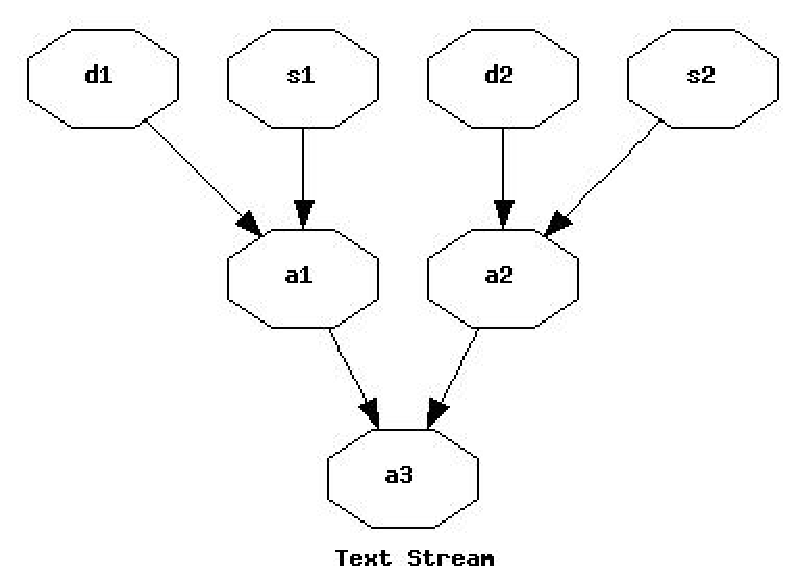
\includegraphics[width=4in]{pedfromstring.eps}%
\lthtmlpictureZ
\lthtmlcheckvsize\clearpage}

\stepcounter{section}
\stepcounter{chapter}
\stepcounter{section}
{\newpage\clearpage
\lthtmlfigureA{xtabular2273}%
\begin{xtabular}{llp{2in}}
	draw\_pedigree & JPG & JPG, PNG, PS \\
	new\_draw\_pedigree & JPG & JPG, PNG, PS \\
	pcolor\_matrix\_pylab & PNG & PNG only \\
	plot\_founders\_by\_year & PNG & PNG only \\
	plot\_founders\_pct\_by\_year & PNG & PNG only \\
	plot\_line\_xy & PNG & PNG only \\
	rmuller\_pcolor\_matrix\_pil & PNG & PNG only \\
	rmuller\_spy\_matrix\_pil & PNG & PNG only \\
	spy\_matrix\_pylab & PNG & PNG only \\
    \end{xtabular}%
\lthtmlfigureZ
\lthtmlcheckvsize\clearpage}

\stepcounter{subsection}
{\newpage\clearpage
\lthtmlpictureA{tex2html_wrap8821}%
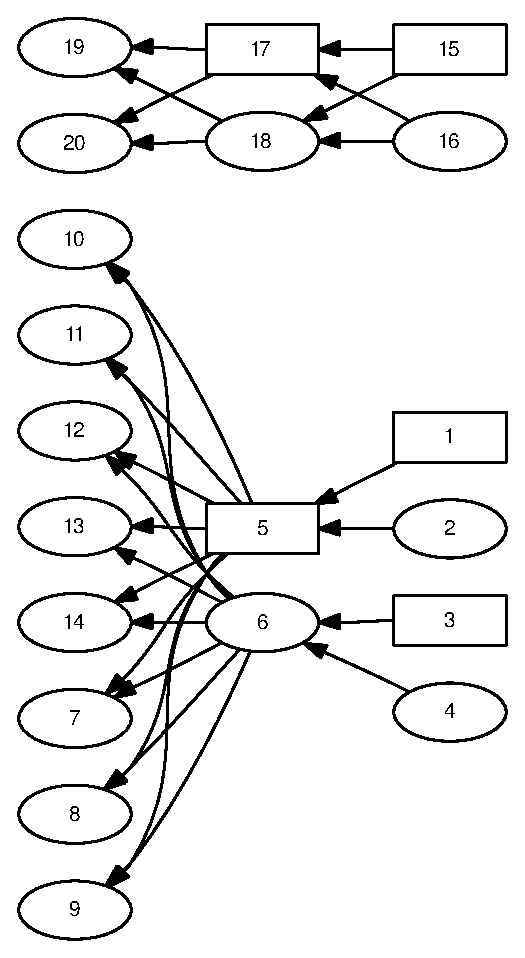
\includegraphics[width=4in]{boichard2Pedigree.eps}%
\lthtmlpictureZ
\lthtmlcheckvsize\clearpage}

{\newpage\clearpage
\lthtmlpictureA{tex2html_wrap8825}%
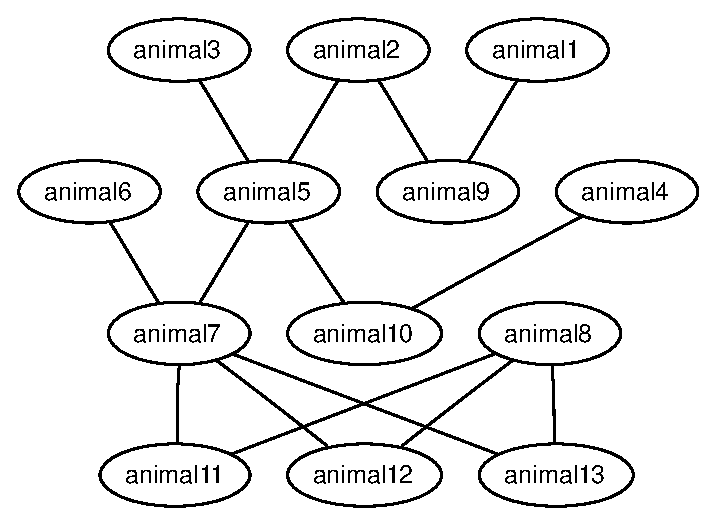
\includegraphics[width=3in]{BoichardPedigreeBasic.eps}%
\lthtmlpictureZ
\lthtmlcheckvsize\clearpage}

{\newpage\clearpage
\lthtmlpictureA{tex2html_wrap8829}%
\includegraphics[width=4in]{dougPRlNotitle.eps}%
\lthtmlpictureZ
\lthtmlcheckvsize\clearpage}

{\newpage\clearpage
\lthtmlpictureA{tex2html_wrap8833}%
\includegraphics[width=4in]{newfoundland.eps}%
\lthtmlpictureZ
\lthtmlcheckvsize\clearpage}

\stepcounter{subsection}
{\newpage\clearpage
\lthtmlpictureA{tex2html_wrap8843}%
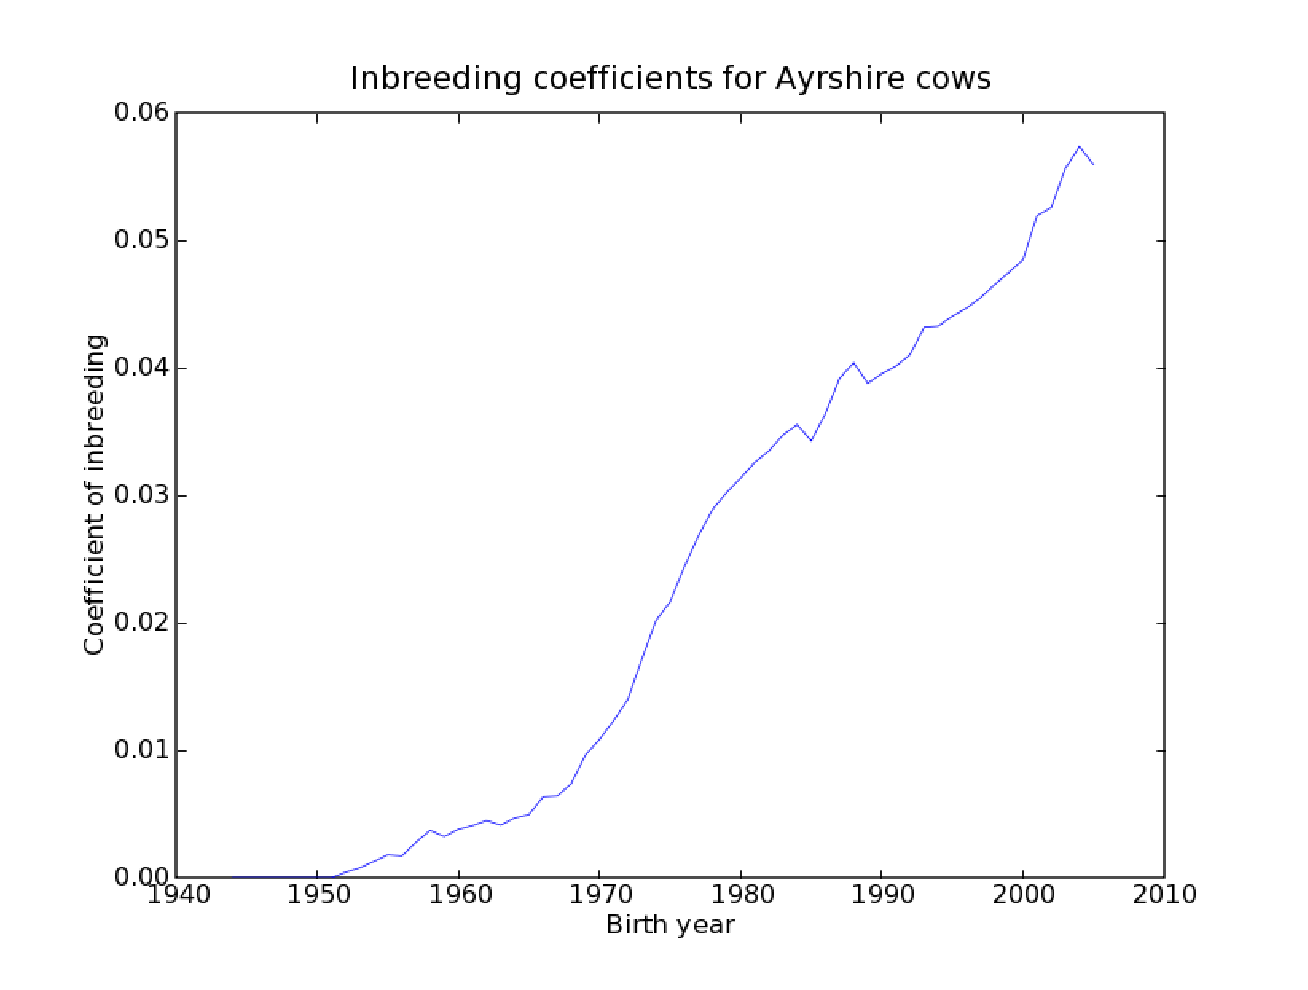
\includegraphics[width=4in]{ayCoiByYear.eps}%
\lthtmlpictureZ
\lthtmlcheckvsize\clearpage}

\stepcounter{subsection}
{\newpage\clearpage
\lthtmlinlinemathA{tex2html_wrap_inline8851}%
$ >1$%
\lthtmlinlinemathZ
\lthtmlcheckvsize\clearpage}

{\newpage\clearpage
\lthtmlinlinemathA{tex2html_wrap_indisplay8853}%
$\displaystyle \scriptsize
\left[ \begin{array}{llllllllllllllllllll}
1. & 0. & 0. & 0. & 0.5 & 0. & 0.25 & 0.25 & 0.25 & 0.25 & 0.25 & 0.25 & 0.25 & 0.25 & 0. & 0. & 0. & 0. & 0. & 0. \\
0. & 1. & 0. & 0. & 0.5 & 0. & 0.25 & 0.25 & 0.25 & 0.25 & 0.25 & 0.25 & 0.25 & 0.25 & 0. & 0. & 0. & 0. & 0. & 0. \\
0. & 0. & 1. & 0. & 0.  & 0.5 & 0.25 & 0.25 & 0.25 & 0.25 & 0.25 & 0.25 & 0.25 & 0.25 & 0. & 0. & 0. & 0. & 0. & 0. \\
0. & 0. & 0. & 1. & 0. & 0.5 & 0.25 & 0.25 & 0.25 & 0.25 & 0.25 & 0.25 & 0.25 & 0.25 & 0. & 0. & 0. & 0. & 0. & 0. \\
0.5 & 0.5 & 0. & 0. & 1. & 0. & 0.5 & 0.5 & 0.5 & 0.5 & 0.5 & 0.5 & 0.5 & 0.5 & 0. & 0. & 0. & 0. & 0. & 0. \\
0. & 0. & 0.5 & 0.5 & 0. & 1. & 0.5 & 0.5 & 0.5 & 0.5 & 0.5 & 0.5 & 0.5 & 0.5 & 0. & 0. & 0. & 0. & 0. & 0. \\
0.25 & 0.25 & 0.25 & 0.25 & 0.5 & 0.5 & 1. & 0.5 & 0.5 & 0.5 & 0.5 & 0.5 & 0.5 & 0.5 & 0. & 0. & 0. & 0. & 0. & 0. \\
0.25 & 0.25 & 0.25 & 0.25 & 0.5 & 0.5 & 0.5 & 1. & 0.5 & 0.5 & 0.5 & 0.5 & 0.5 & 0.5 & 0. & 0. & 0. & 0. & 0. & 0. \\
0.25 & 0.25 & 0.25 & 0.25 & 0.5 & 0.5 & 0.5 & 0.5 & 1. & 0.5 & 0.5 & 0.5 & 0.5 & 0.5 & 0. & 0. & 0. & 0. & 0. & 0. \\
0.25 & 0.25 & 0.25 & 0.25 & 0.5 & 0.5 & 0.5 & 0.5 & 0.5 & 1. & 0.5 & 0.5 & 0.5 & 0.5 & 0. & 0. & 0. & 0. & 0. & 0. \\
0.25 & 0.25 & 0.25 & 0.25 & 0.5 & 0.5 & 0.5 & 0.5 & 0.5 & 0.5 & 1. & 0.5 & 0.5 & 0.5 & 0. & 0. & 0. & 0. & 0. & 0. \\
0.25 & 0.25 & 0.25 & 0.25 & 0.5 & 0.5 & 0.5 & 0.5 & 0.5 & 0.5 & 0.5 & 1. & 0.5 & 0.5 & 0. & 0. & 0. & 0. & 0. & 0. \\
0.25 & 0.25 & 0.25 & 0.25 & 0.5 & 0.5 & 0.5 & 0.5 & 0.5 & 0.5 & 0.5 & 0.5 & 1. & 0.5 & 0. & 0. & 0. & 0. & 0. & 0. \\
0.25 & 0.25 & 0.25 & 0.25 & 0.5 & 0.5 & 0.5 & 0.5 & 0.5 & 0.5 & 0.5 & 0.5 & 0.5 & 1. & 0. & 0. & 0. & 0. & 0. & 0. \\
0. & 0. & 0. & 0. & 0. & 0. & 0. & 0. & 0. & 0. & 0. & 0. & 0. & 0. & 1. & 0. & 0.5 & 0.5 & 0.5 & 0.5 \\
0. & 0. & 0. & 0. & 0. & 0. & 0. & 0. & 0. & 0. & 0. & 0. & 0. & 0. & 0. & 1. & 0.5 & 0.5 & 0.5 & 0.5 \\
0. & 0. & 0. & 0. & 0. & 0. & 0. & 0. & 0. & 0. & 0. & 0. & 0. & 0. & 0.5 & 0.5 & 1. & 0.5 & 0.75 & 0.75 \\
0. & 0. & 0. & 0. & 0. & 0. & 0. & 0. & 0. & 0. & 0. & 0. & 0. & 0. & 0.5 & 0.5 & 0.5 & 1. & 0.75 & 0.75 \\
0. & 0. & 0. & 0. & 0. & 0. & 0. & 0. & 0. & 0. & 0. & 0. & 0. & 0. & 0.5 & 0.5 & 0.75 & 0.75 & 1.25 & 0.75 \\
0. & 0. & 0. & 0. & 0. & 0. & 0. & 0. & 0. & 0. & 0. & 0. & 0. & 0. & 0.5 & 0.5 & 0.75 & 0.75 & 0.75 & 1.25
\end{array} \right]
\normalsize
$%
\lthtmlindisplaymathZ
\lthtmlcheckvsize\clearpage}

{\newpage\clearpage
\lthtmlpictureA{tex2html_wrap8857}%
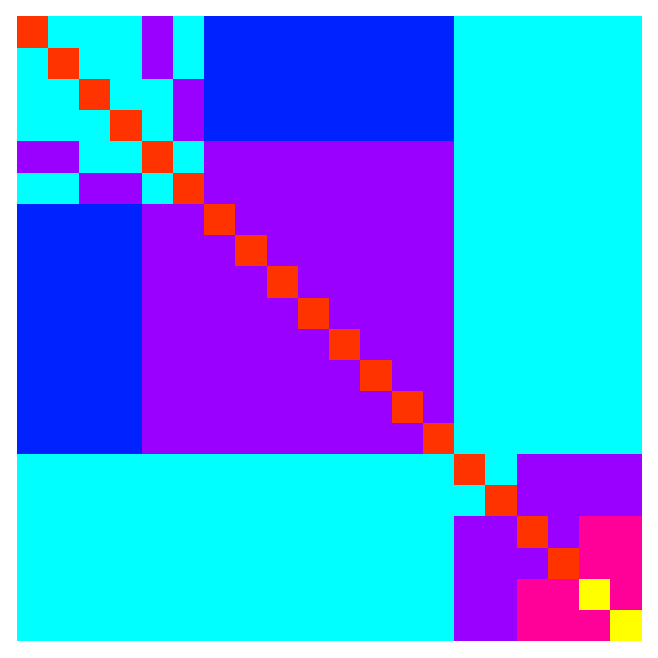
\includegraphics[width=3in]{boichard2Pcolor.eps}%
\lthtmlpictureZ
\lthtmlcheckvsize\clearpage}

{\newpage\clearpage
\lthtmlpictureA{tex2html_wrap8861}%
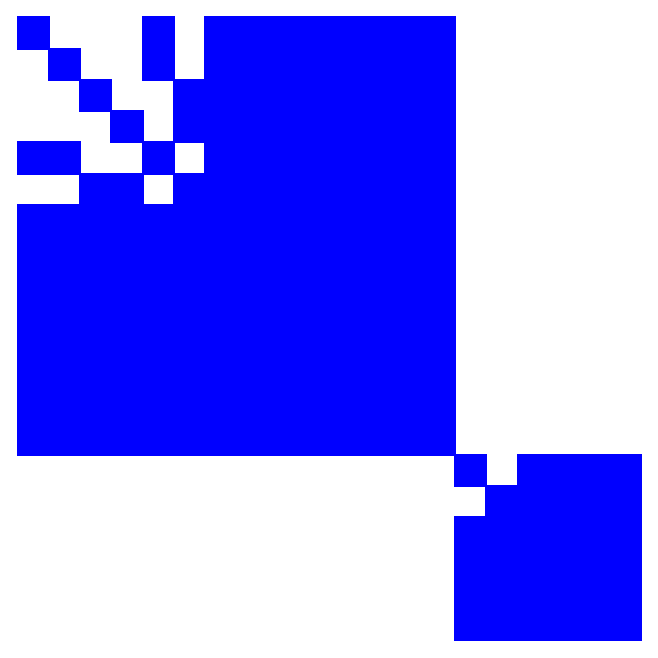
\includegraphics[width=3in]{boichard2Spy.eps}%
\lthtmlpictureZ
\lthtmlcheckvsize\clearpage}

\stepcounter{chapter}
\stepcounter{section}
{\newpage\clearpage
\lthtmlfigureA{xtabular2494}%
\begin{xtabular}{llp{2.5in}}
	age           &   real          &  Age of animal \\
	alive         &   char(1)       &  Animal's mortality status \\
	ancestor      &   char(1)       &  Ancestor status \\
	animalID      &   integer       &  \textbf{Must be unique!} \\
	animalName    &   varchar(128)  &  Animal name \\
	birthyear     &   integer       &  Birth year \\
	breed         &   text          &  Breed \\
	coi           &   real          &  Coefficient of inbreeding \\
	damID         &   integer       &  Dam's ID \\
	founder       &   char(1)       &  Founder status \\
	gencoeff      &   real          &  Pattie's generation coefficient \\
	generation    &   real          &  Generation \\
	herd          &   integer       &  Herd ID \\
	infGeneration &   real          &  Inferred generation \\
	num\_daus     &   integer       &  Number of daughters \\
	num\_sons     &   integer       &  Number of sons \\
	num\_unk      &   integer       &  Offspring of unknown sex \\
	originalHerd  &   varchar(128)  &  Original herd ID \\
	originalID    &   text          &  Animal's original ID \\
	pedgreeComp   &   real          &  Pedigree completeness \\
	renumberedID  &   integer       &  Animal's renumbered ID \\
	sex           &   char(1)       &  Sex of animal \\
	sireID        &   integer       &  Sire's ID \\
    \end{xtabular}%
\lthtmlfigureZ
\lthtmlcheckvsize\clearpage}

\stepcounter{subsection}
{\newpage\clearpage
\lthtmlpictureA{tex2html_wrap8870}%
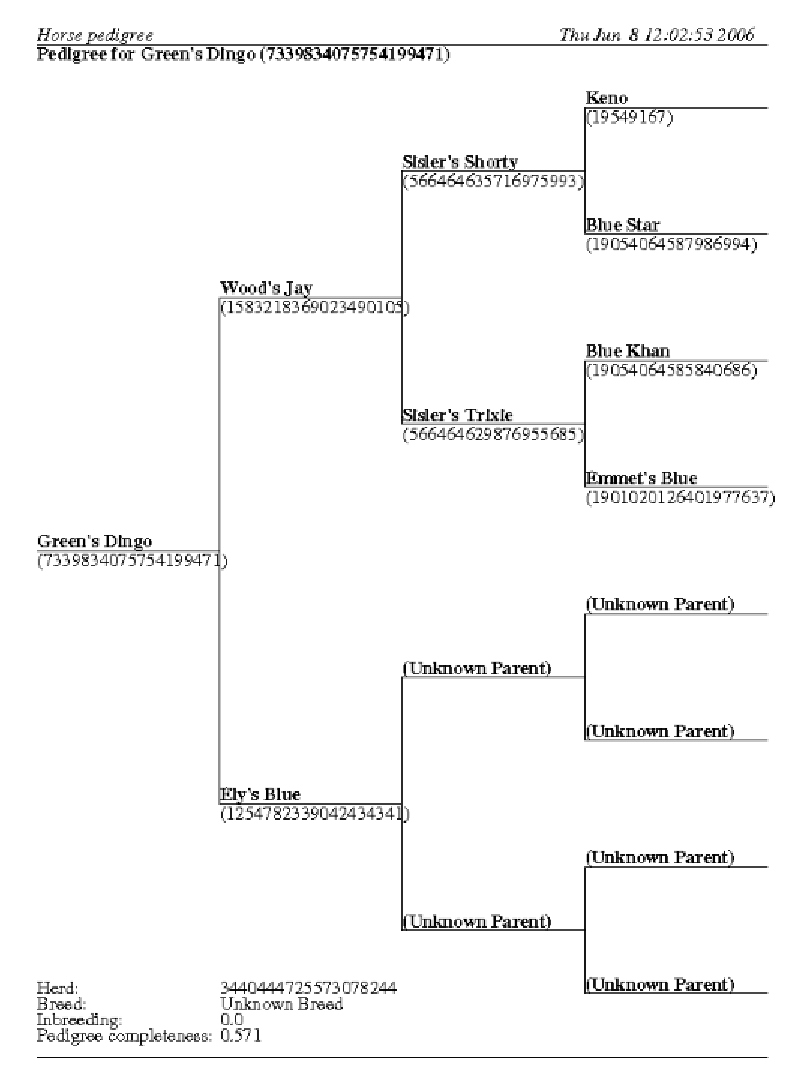
\includegraphics[width=6in]{greensDingoPedigree.eps}%
\lthtmlpictureZ
\lthtmlcheckvsize\clearpage}

\stepcounter{section}
\stepcounter{section}
\stepcounter{chapter}
\stepcounter{section}
\stepcounter{subsection}
\stepcounter{section}
\stepcounter{section}
{\newpage\clearpage
\lthtmlpictureA{tex2html_wrap8891}%
\includegraphics[width=6in]{BoichardPedigreeColored.eps}%
\lthtmlpictureZ
\lthtmlcheckvsize\clearpage}

\stepcounter{section}
\stepcounter{chapter}
\appendix
\stepcounter{chapter}
{\newpage\clearpage
\lthtmlfigureA{xtabular2725}%
\begin{xtabular}{l|p{1in}|p{1in}|p{3in}}
    new\_amatrix.py & new\_amatrix.ini & new\_amatrix.ped & Create, save, load, and view information about NewAMatrix objects \\
    new\_classes.py & new\_classes.ini & boichard2.ped & ??? \\
    new\_db.py & new\_db.ini & hartlandclark.ped & Loading a pedigree into SQLite and creating a report of mean inbreeeding by birth year \\
    new\_doug.py & new\_doug.ini & doug.ped & Reading a pedigree in which names are strings, drawing pedigrees \\
    new\_format.py & new\_format.ini & boichard2a.ped & Reading a pedigree using the `skip column' format code (Z), printing pedigree metadata \\
    new\_graphics.py & new\_graphics.ini & boichard2.ped & Use of a number of routines from \module{pyp_graphics} \\
    new\_hartl.py & new\_hartl.ini & hartlandclark.ped & Demonstrates use of \function{pyp_graphics.draw_pedigree()} \\
    new\_ids.py & new\_ids.ini & new\_ids2.ped & Demonstrates reading tab-delimited files, using strings as animal IDs, overriding the default missing parent code, printing animal records \\
    new\_inbreeding.py & new\_inbreeding.ini & new\_renumbering.ped & Calculating coefficients of inbreeding \\
    new\_inbreeding2.py & new\_inbreeding2.ini, new\_inbreeding2multiple.ini & new\_renumbering.ped, horse.ped & Advanced .ini file techniques, computations on extremely inbred animals, calculation of summary statistics for coefficients of relationship \\
    new\_jbc.py & new\_jbc.ini & new\_ids2.ped & Using \function{pyp_jbc.color_pedigree()} to produce a weighted, colored pedigree \\
    new\_lacy.py & new\_lacy.ini, new\_format.ini & new\_lacy.ped, boichard2a.ped & Calculating effective ancestor and founder numbers \\
    new\_methods.py & new\_format.ini & boichard2a.ped & Use of \function{pyp_metrics.related\_animals()} and \function{pyp_metrics.common\_ancestors()} \\
    new\_networkx.py & new\_networkx.ini & generations.ped & Use of [algebraic] graph functions \\
    new\_options.py & new\_options.ini & new\_lacy.ped & Use of the configuration files \\
    new\_renumbering.py & new\_renumbering.ini & new\_renumbering.ped & Renumbering a pedigree, calculating inbreeding, pedigree drawing \\
    new\_reporting.py & new\_reporting.ini & new\_renumbering.ped & Use of reporting functions \\
    new\_simulate.py & new\_simulate.ini & None & Demonstrates how to create a random pedigree and produce a drawing of that pedigree. \\
    \end{xtabular}%
\lthtmlfigureZ
\lthtmlcheckvsize\clearpage}

\stepcounter{chapter}
{\newpage\clearpage
\lthtmlfigureA{xtabular2755}%
\begin{xtabular}{l|p{1in}|p{3in}}
    Fam_Record & {FAM} & Alphanumeric with underscores; formed from parent IDs \\
     & {HUSB} & Sire, if known \\
     & {WIFE} & Dam, if known \\
     & {CHIL} & Pointer to Individual_Record (one record per child) \\
    Individual_Record & {INDI} & Individual ID \\
     & SEX & M, F, or U (unknown) \\
     & NAME & Individual's name, if known \\
     & BIRT & Indicates that a birth date or year follows \\
     & DATE & Birth date or birth year, if known \\
     & FAMC & Pointer to family to which this individual belongs \\
     & FAMS & Pointer to family in which this individual is a parent \\
    \end{xtabular}%
\lthtmlfigureZ
\lthtmlcheckvsize\clearpage}

{\newpage\clearpage
\lthtmlfigureA{xtabular2776}%
\begin{xtabular}{l|p{1in}|p{3in}}
    Header & {HEAD} & --- \\
     & {SOUR} & {PYPEDAL} \\
     & {VERS} & V2.0 \\
     & {CORP} & {USDA-ARS-BA-ANRI-AIPL} \\
     & {DEST} & {PYPEDAL} \\
     & {DATE} & Timestamp from time of file creation \\
     & {FILE} & Filename provided by user \\
     & {GEDC} & --- \\
     & {VERS} & {VERS 5.5} \\
     & {FORM} & Lineage-Linked \\
     & {CHAR} & {ASCII} \\
    Fam_Record & {FAM} & Alphanumeric with underscores; formed from parent IDs \\
     & {HUSB} & Sire, if known \\
     & {WIFE} & Dam, if known \\
     & {CHIL} & Pointer to Individual_Record (one record per child) \\
    Individual_Record & {INDI} & Individual ID \\
     & SEX & M, F, or U (unknown) \\
     & NAME & Individual's name, if known \\
     & BIRT & Indicates that a birth date or year follows \\
     & DATE & Birth date or birth year, if known \\
     & FAMC & Pointer to family to which this individual belongs \\
     & FAMS & Pointer to family in which this individual is a parent \\
    \end{xtabular}%
\lthtmlfigureZ
\lthtmlcheckvsize\clearpage}


\end{document}
